\section{Overview}
The BioQuick module serves as a critical interface for SPI communication, enabling configuration of an ADC SAR and retrieval of analog-to-digital conversion values with support for read/write operations across multiple memory addresses utilizing an auto-incremental addressing. This module ensures efficient data handling and seamless integration within a larger system by bridging low-frequency SPI interactions and high-frequency memory access operations.

To provide a clear understanding of the structure of the digital system, a simplified block diagram is presented early in Fig.~\ref{fig:overview}. This diagram illustrates the interaction between the SPI Interface, Synchronizer, and APB Master, highlighting the data flow across the low-frequency (1 MHz) and high-frequency (100 MHz) domains, and offering a visual context for the module's operation before delving into detailed descriptions of additional components.

\begin{figure}[!htb]
    \centering
    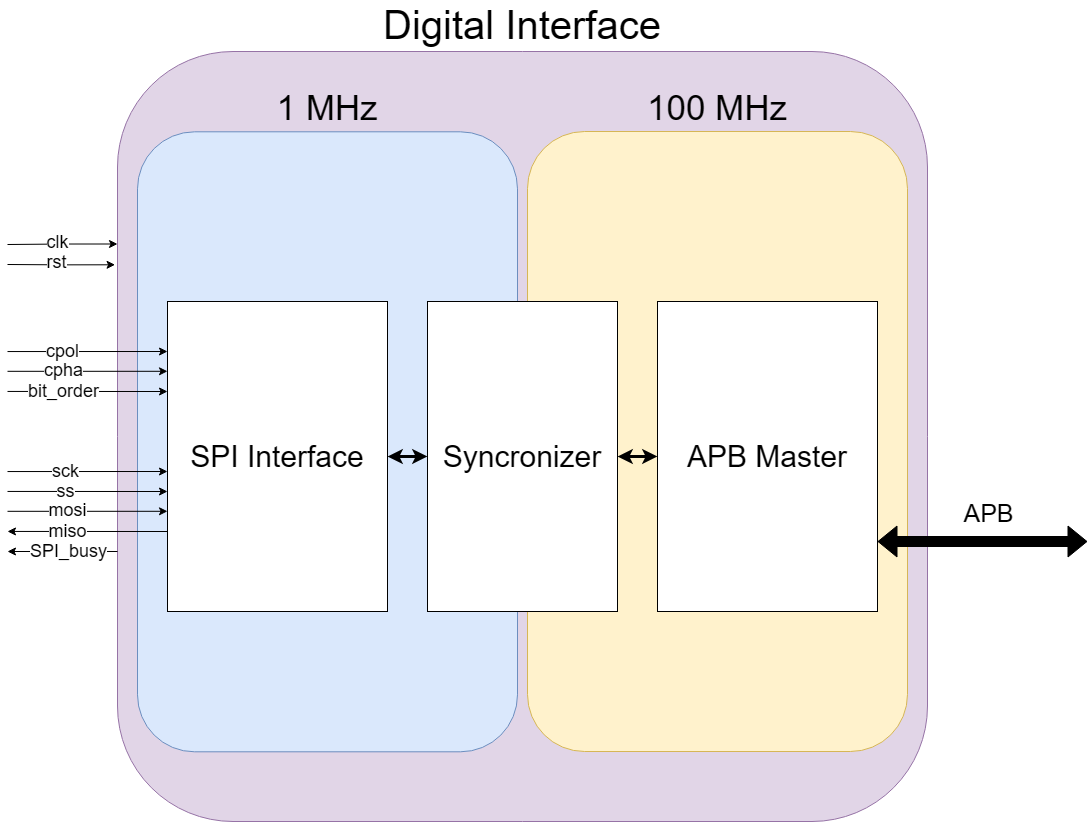
\includegraphics[width=1\linewidth]{figures/overview.png}
    \caption{Simplified system overview}
    \label{fig:overview}
\end{figure}

% Low-frequency modules
The low-frequency components, operating at up to 1 MHz, are responsible for managing SPI communication with an external master. Their primary role is to handle data transfer by converting between serial and parallel formats and ensuring data integrity through CRC validation and generation. Fig.~\ref{fig:low-freq} provides a detailed block diagram of the low-frequency side, inspired by the structured visual style seen in other system diagrams.

\begin{figure}[!htb]
    \centering
    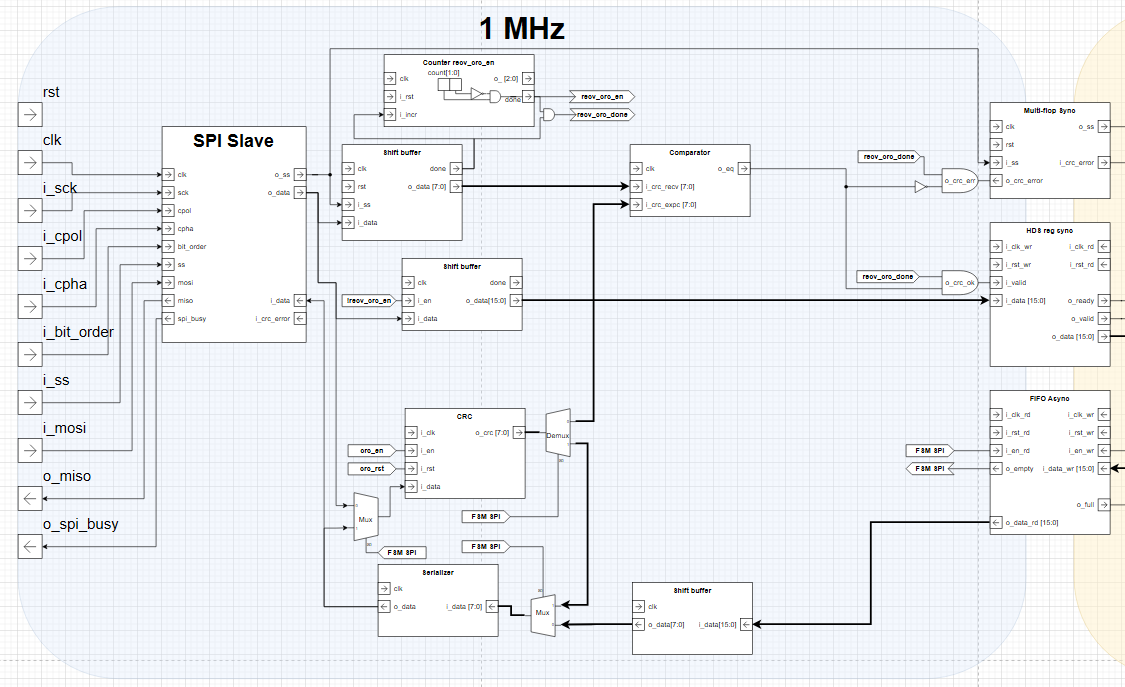
\includegraphics[width=1\linewidth]{figures/low_freq.png}
    \caption{Low-frequency block diagram}
    \label{fig:low-freq}
\end{figure}

These components include:
\begin{itemize}[nosep]
    \item \textbf{SPI Slave Interface}: Manages communication with the external SPI Master, supporting read/write transactions with configuration inputs (cpol, cpha, bit\_order), clocks (clk, sck), reset, transaction signals (i\_ss, i\_mosi, o\_miso), and status output (spi\_busy).
    \item \textbf{Deserializer}: Converts serial data received via SPI (i\_mosi) into parallel data for internal processing, supporting MSB/LSB order and burst data handling.
    \item \textbf{Serializer}: Converts parallel data to serial data for SPI transmission (o\_miso), also supporting MSB/LSB order and burst data.
    \item \textbf{CRC Block}: Implements the CRC\&CCITT algorithm for error correction, validating incoming data during write operations and generating CRC for outgoing data during read operations.
\end{itemize}

These blocks ensure reliable data transfer adhering to project constraints like a single CRC block and a specific data format (4-bit operation field with 1 bit for operation type extended by 3 zeros, 12-bit address, 16-bit data, 8-bit CRC), meeting the performance target of up to 1 MHz as per the proposal.

% High-frequency modules
The high-frequency components, operating at 100 MHz, focus on efficient memory access and data processing with robust synchronization. Their role is to manage address organization and communication protocols for seamless memory operations. Fig.~\ref{fig:high-freq} provides a detailed block diagram of the high-frequency side.

\begin{figure}[!htb]
    \centering
    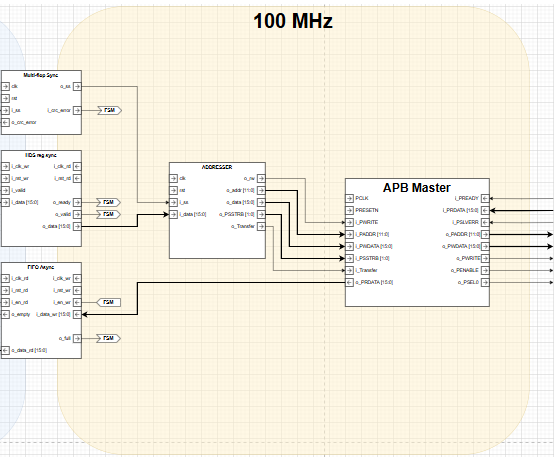
\includegraphics[width=1\linewidth]{figures/high_freq.png}
    \caption{High-frequency block diagram}
    \label{fig:high-freq}
\end{figure}

These components include:
\begin{itemize}[nosep]
    \item \textbf{Addresser}: Reorganizes 16-bit data packages into a format compatible with the APB Master, calculating address auto-increment as required.
    \item \textbf{APB Master}: Commands communication with the APB Slave to perform write or read operations on memory addresses.
    \item \textbf{APB Slave}: Executes memory access operations under the APB Master’s direction (outside deliverable scope but included for validation).
\end{itemize}
